\documentclass[conference,a4paper]{IEEEtran}
\usepackage{cite}
\usepackage{amsmath,amssymb,amsfonts}
\usepackage{graphicx}
\usepackage{textcomp}
\usepackage{xcolor}
\usepackage{booktabs}
\usepackage{tikz}
\usetikzlibrary{arrows.meta, positioning, shapes.geometric, fit, calc}
\usepackage[hidelinks]{hyperref}

\begin{document}

\title{Visual Dock-Velocity Feedforward for ROV Docking to a Moving Station: Failure Mechanism, Feedforward Redesign and Estimator Robustness}

\author{\IEEEauthorblockN{1\textsuperscript{st} Chak Wang Choi}
\IEEEauthorblockA{\textit{School of Mechanical and Manufacturing Engineering} \\
\textit{UNSW Sydney}\\
Sydney, Australia \\
z5413670@ad.unsw.edu.au}
\and
\IEEEauthorblockN{2\textsuperscript{nd} William J.B. Midgley}
\IEEEauthorblockA{\textit{School of Mechanical and Manufacturing Engineering} \\
\textit{UNSW Sydney}\\
Sydney, Australia \\
w.midgley@unsw.edu.au\\
ORCID: 0000-0003-3786-1691}
}

\maketitle

\begin{abstract}
Moored and suspended docking stations move with the waves, so the terminal visual stage of underwater docking must track a moving target. The natural extension of a static-dock pipeline is to estimate the dock velocity onboard and feed it forward into the vehicle command. We report what happened when that was done for a passive-marker docking stage on a low-cost ROV in simulation with the production autopilot in the loop: a reactive baseline docks at every sway period, while a constant-velocity estimator with velocity feedforward fails at the 8 and 6~s periods of the intended site, and its own signals blame the estimator. Rebuilding every measurement from the recorded trials shows the estimate is accurate and the failure is control: the feedforward over-drives a plant whose identified gain is 2.7 against the 1.3 to 1.6 it was tuned to, and the apparent phantom velocity is dead-reckoning during the marker blackout the over-swing causes. An oracle feedforward from the true dock velocity over-swings identically, placing the limit in the open-loop law. Closing the feedforward as a body-velocity setpoint on the navigation velocity, with a bounded velocity state during blackout, removes the over-swing at every period and docks cleanly from 20 to 8~s across an 82-trial, four-arm sweep, with entry-plane offsets under 2~cm. Under first-order Gauss-Markov navigation error, world-frame and relative-frame estimators both absorb a slow velocity bias one for one; the relative frame removes only the fast error, and the velocity loop is what cancels the bias.
\end{abstract}

\begin{IEEEkeywords}
underwater docking, remotely operated vehicle, visual servoing, moving target, Kalman filter, velocity feedforward, plant identification
\end{IEEEkeywords}

\section{Introduction}
\label{sec:intro}

Docking gives a resident underwater vehicle a place to recharge and offload data without surfacing, and it removes the slow, weather-limited and expensive recovery by a support vessel from the mission cycle. The risk concentrates in the final metres, where the vehicle flies onto the station on its forward camera. Real stations are not still. A tether management system suspended from a vessel follows the vessel's heave: in the only reported autonomous docking to such a cage, the cage moved 1.1~m peak to peak at 8.5~s \cite{trslic2020vision}. A moored station follows the wave orbital motion at its depth, which decays exponentially with depth at a rate set by the wave period, so long swell reaches a dock at continental-shelf depth with displacements of order 0.1~m while short wind sea does not \cite{holthuijsen2007waves}. Off New South Wales, the operating context of this work, the mean sea state is 1.6~m at 8~s \cite{short1992wave,kinsela2024nearshore}, which forces a 0.1~m sway on a dock near 33~m depth.

The docking control literature treats the dock as a fixed pose and its estimator as a noise filter. Trslic et al.\ servoed reactively on the latest measured pose and accepted contact during dynamic docking \cite{trslic2020vision}; their later heave predictor used a pressure sensor on the cage and was evaluated offline \cite{trslic2020neuro}. Recent marker-based systems fuse the camera pose with an extended Kalman filter but keep the dock frame as the world frame \cite{gunzel2026docking,ni2025vision}. The obvious extension for a moving station is to estimate the dock velocity onboard and feed it forward into the vehicle command, so that the vehicle rides along with the dock and the position loop only trims the residual. To our knowledge no prior work closes that loop through vision alone.

This paper reports what happens when the obvious extension is added to a passive-marker terminal docking stage for a low-cost ROV. In simulation with the production autopilot in the loop, a reactive baseline docks cleanly onto a station swaying with 0.1~m amplitude down to 8~s periods, whereas a constant-velocity estimator with velocity feedforward degrades at 10~s and fails at 8 and 6~s. The estimator's own signals point at itself: its velocity state reaches many times the true dock amplitude in the failed trials. Rebuilding every measurement from the recorded trials shows that this reading is wrong, and the paper's contributions follow from what the data show instead:
\begin{enumerate}
  \item a failure mechanism established from the recorded trials rather than from the system's own diagnostics: the dock measurement and the velocity estimate are accurate, the feedforward over-drives a plant whose gain and lag differ from those it was tuned to, and the estimator's apparent runaway is dead-reckoning during the marker blackout that the over-swing causes;
  \item a redesigned feedforward that closes on the vehicle's own velocity, with a bounded velocity state during blackout, evaluated against the reactive baseline, the original method and an oracle feedforward from ground-truth dock velocity, which separates estimator-limited from plant-limited failure;
  \item an observability result for the estimator under correlated navigation error: a camera measuring relative position cannot distinguish a slowly varying vehicle-velocity error from dock velocity, for a world-frame or a relative-frame estimator alike, and only the fast part of the error is removed by estimating in the relative frame.
\end{enumerate}

Section~\ref{sec:related} places the work, Section~\ref{sec:system} describes the system, Section~\ref{sec:failure} establishes the mechanism, Section~\ref{sec:redesign} gives the redesign, Section~\ref{sec:design} the experiments, and Sections~\ref{sec:results} to~\ref{sec:conclusion} the results and what they mean for a deployment.

\section{Related Work}
\label{sec:related}

Placeholder, budget 0.75 page, about 600 words compressed from the thesis literature review. Three paragraphs: docking with moving stations (Trslic 2020 vision and neuro-fuzzy papers, Guo 2024 suspended dock dynamics, Morinaga 2021, Gunzel 2026); target tracking with correlated measurement error and relative-frame estimation (Bar-Shalom, Li and Jilkov, the relative navigation literature); visual servoing on moving targets and the effect of loop latency (Chaumette and Hutchinson, Corke and Good). Acoustic and electromagnetic homing, image formation and fiducial marker surveys are omitted.

\section{System}
\label{sec:system}

Placeholder, budget 1 page. Condensed from the thesis architecture and Part A methodology. Simulation stack (Gazebo, ArduSub software-in-the-loop, BlueROV2 Heavy, prescribed dock motion), the size-graded marker set in two sentences, fusion, the nine-state error-state filter with its two regimes, guidance and the two controllers, the feedforward path, and the state machine. State explicitly that the vehicle pose in simulation is Gazebo ground truth relayed into the transform tree, since Section~\ref{sec:failure} depends on it.

\begin{figure*}[t]
  \centering
  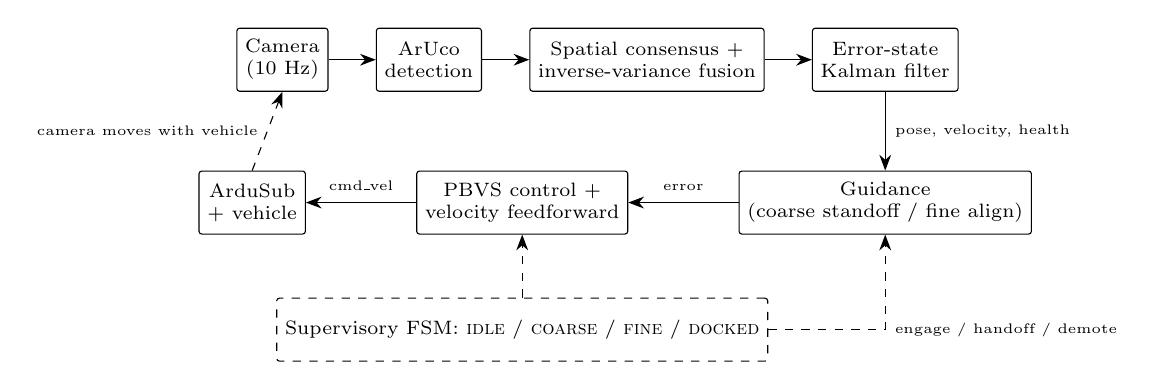
\begin{tikzpicture}[font=\scriptsize, >={Stealth[length=2mm]},
    box/.style={draw, rounded corners=1pt, align=center, minimum height=8mm, inner sep=3pt}]
    \node[box] (cam) {Camera\\(10~Hz)};
    \node[box, right=6mm of cam] (det) {ArUco\\detection};
    \node[box, right=6mm of det] (fus) {Spatial consensus +\\inverse-variance fusion};
    \node[box, right=6mm of fus] (kf) {Error-state\\Kalman filter};
    \node[box, below=10mm of kf] (guid) {Guidance\\(coarse standoff / fine align)};
    \node[box, left=14mm of guid] (ctl) {PBVS control +\\velocity feedforward};
    \node[box, left=14mm of ctl] (veh) {ArduSub\\+ vehicle};
    \node[box, below=8mm of ctl, dashed] (fsm) {Supervisory FSM: \textsc{idle} / \textsc{coarse} / \textsc{fine} / \textsc{docked}};
    \draw[->] (cam) -- (det);
    \draw[->] (det) -- (fus);
    \draw[->] (fus) -- (kf);
    \draw[->] (kf) -- node[right]{\tiny pose, velocity, health} (guid);
    \draw[->] (guid) -- node[above, yshift=1pt]{\tiny error} (ctl);
    \draw[->] (ctl) -- node[above, yshift=1pt]{\tiny cmd\_vel} (veh);
    \draw[dashed, ->] (veh.north) -- node[left]{\tiny camera moves with vehicle} (cam.south);
    \draw[dashed, ->] (fsm.north) -- (ctl.south);
    \draw[dashed, ->] (fsm.east) -| node[right]{\tiny engage / handoff / demote} (guid.south);
  \end{tikzpicture}

  \caption{System architecture. The state machine gates the controllers on the filter's health signal; the dashed vehicle-to-camera path is the coupling examined in Section~\ref{sec:failure}.}
  \label{fig:arch}
\end{figure*}

\begin{figure*}[t]
  \centering
  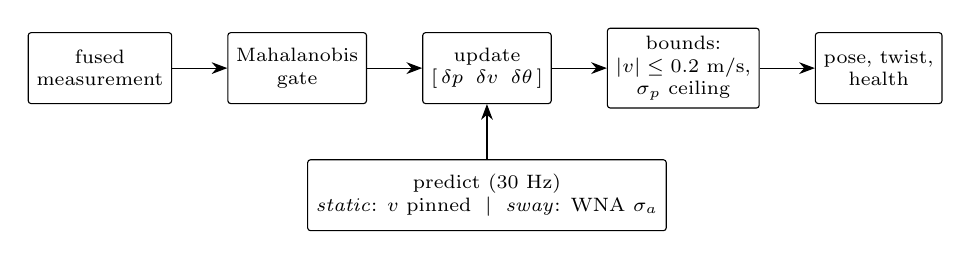
\begin{tikzpicture}[font=\scriptsize, >={Stealth[length=2mm]},
  box/.style={draw, rounded corners=1pt, align=center, minimum height=9mm, inner sep=3pt}]
  \node[box] (meas) {fused\\measurement};
  \node[box, right=7mm of meas] (gate) {Mahalanobis\\gate};
  \node[box, right=7mm of gate] (upd) {update\\ $[\,\delta p \;\; \delta v \;\; \delta\theta\,]$};
  \node[box, right=7mm of upd] (bound) {bounds:\\ $|v| \leq 0.2$ m/s,\\ $\sigma_p$ ceiling};
  \node[box, right=7mm of bound] (out) {pose, twist,\\health};
  \node[box, below=7mm of upd] (pred) {predict (30 Hz)\\ \emph{static}: $v$ pinned $\;|\;$ \emph{sway}: WNA $\sigma_a$};
  \draw[->] (meas) -- (gate);
  \draw[->] (gate) -- (upd);
  \draw[->] (upd) -- (bound);
  \draw[->] (bound) -- (out);
  \draw[->] (pred) -- (upd);
\end{tikzpicture}

  \caption{Filter structure: the nine-state error-state filter with the two process-noise regimes, the measurement gate and the state bounds.}
  \label{fig:kf}
\end{figure*}

\section{Failure Mechanism}
\label{sec:failure}

Placeholder, budget 1.25 pages. The docking envelope sweep (Fig.~\ref{fig:pdock}), the failed 8~s trial (Fig.~\ref{fig:trajectory}), and the offline decomposition of the recorded trials (Fig.~\ref{fig:mech}): the world-frame measurement is within 1~cm of truth, the velocity state is accurate while markers are visible, the feedforward over-drives the plant with the identified gain and lag, and the blackout dead-reckoning that produces the apparent phantom velocity. The loop argument uses the plant gain and lag identified in the step tests.

\begin{figure}[t]
  \centerline{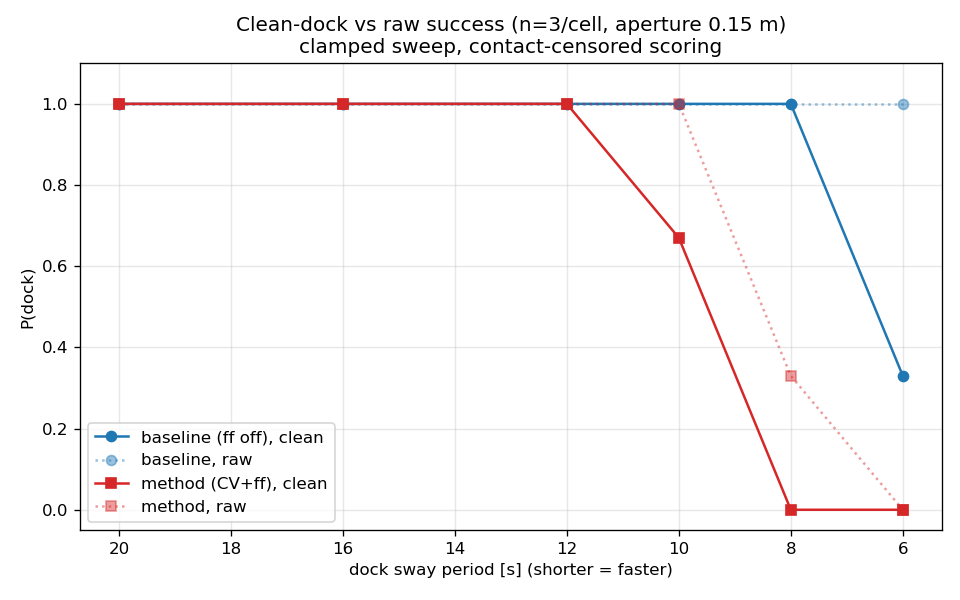
\includegraphics[width=0.7\columnwidth]{figures/clean_pdock.png}}
  \caption{Docking success versus sway period, reactive baseline versus constant-velocity filter with feedforward; raw (dotted) and contact-censored (solid) scoring.}
  \label{fig:pdock}
\end{figure}

\begin{figure}[t]
  \centerline{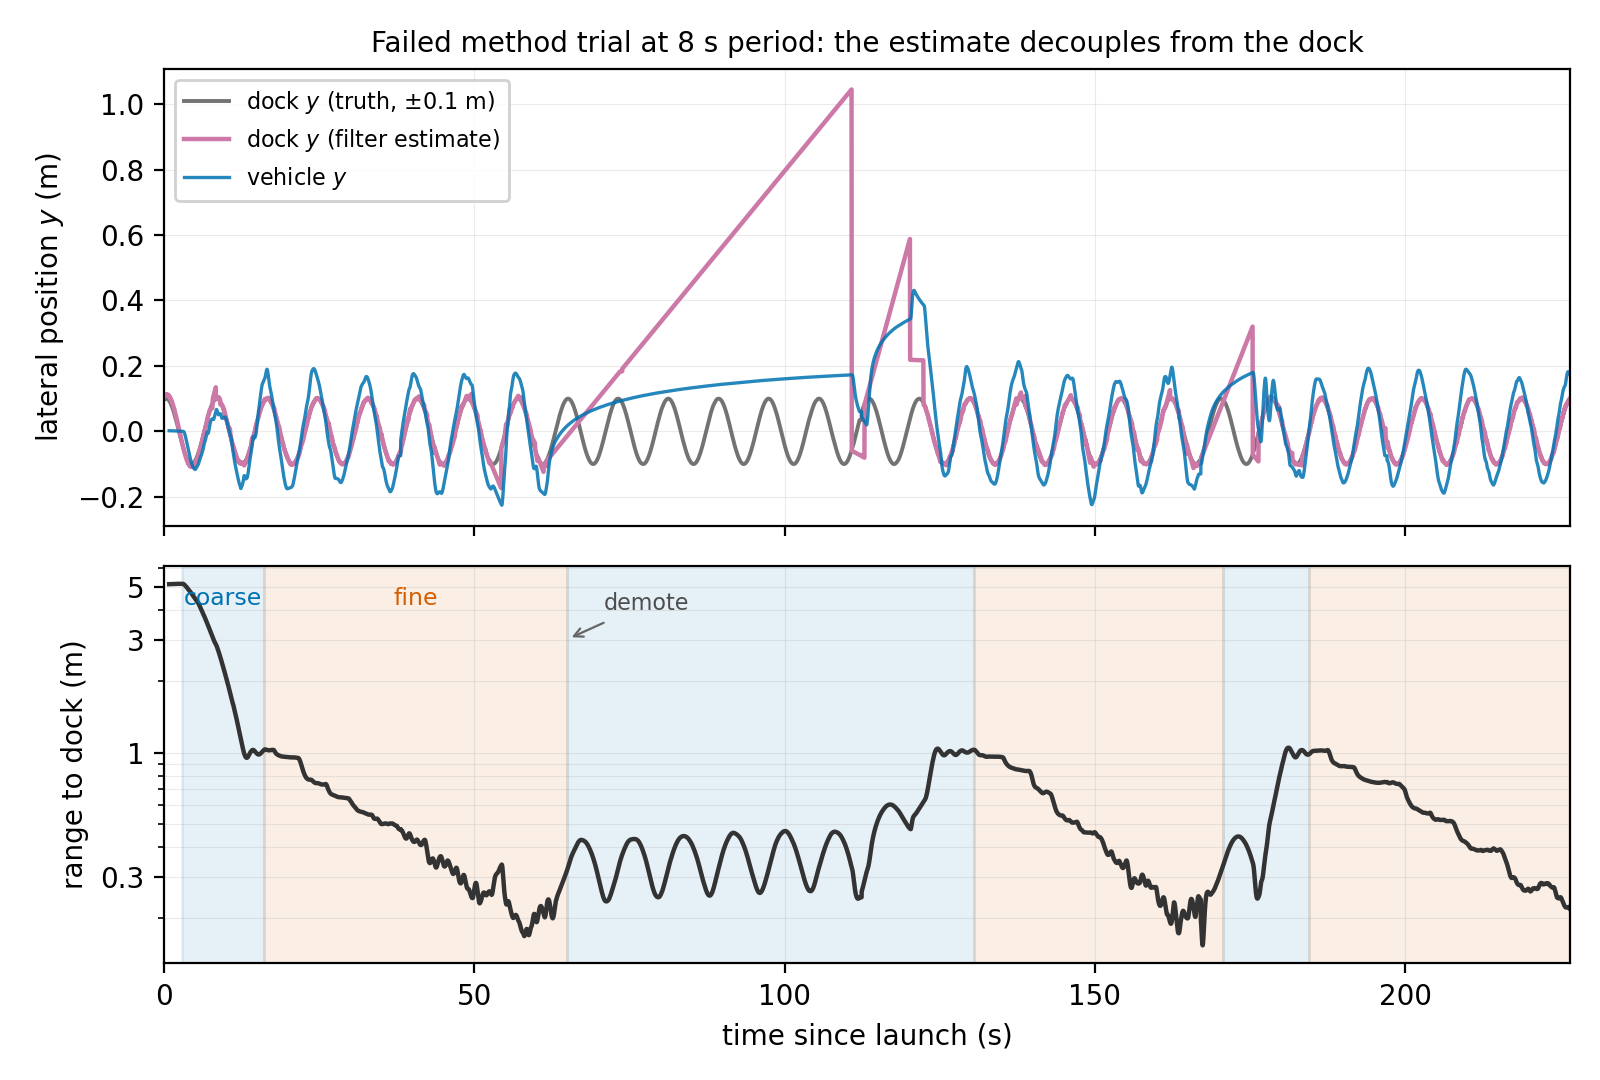
\includegraphics[width=0.75\columnwidth]{figures/rov_trajectory_failure.png}}
  \caption{Failed feedforward trial at 8~s. Top: lateral position of the true dock, the estimate and the vehicle. Bottom: range to the dock with phases shaded.}
  \label{fig:trajectory}
\end{figure}

\begin{figure}[t]
  \centerline{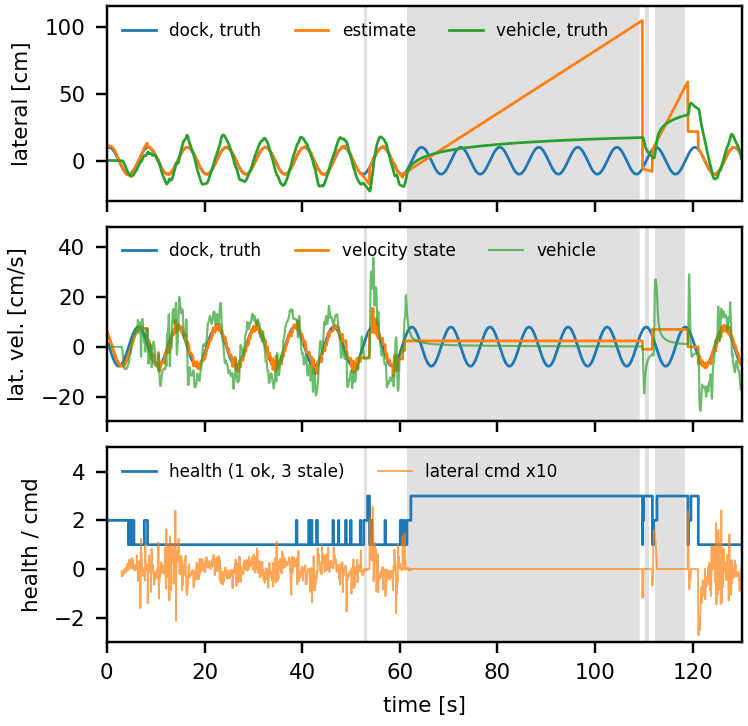
\includegraphics[width=0.95\columnwidth]{figures/mechanism_p8.png}}
  \caption{Decomposition of the failed 8~s trial. Top: the estimate sits on the dock while the vehicle over-swings, then dead-reckons when markers are lost (shaded). Middle: the velocity state tracks the true dock velocity; the vehicle's is twice it. Bottom: filter health and lateral command; the command is zero throughout the blackout.}
  \label{fig:mech}
\end{figure}

% This section presumes the control-first decision on the fix arm (issue
% UNSWROV/bluerov2-docking#67): a velocity-closed feedforward plus a bounded
% velocity state, with the relative-frame estimator in a supporting role. If
% that decision changes, rewrite this section and Section VI's arm table.
\section{Feedforward Redesign and Estimator}
\label{sec:redesign}

Section~\ref{sec:failure} locates the failure in the path from the estimated dock velocity to the vehicle's response, and in what the estimator does while it has no measurements. The redesign evaluated as arm C therefore changes those two things and nothing else.

\subsection{Velocity-closed feedforward}

The original method adds $K_{ff}\,\hat{v}_d$ directly to an effort-like command, so the vehicle's velocity response is $K_{ff}\,g$ times the dock velocity for whatever plant gain $g$ the mode and the trim happen to produce. The redesign treats the sum of the feedback command and the rotated dock velocity as a body-frame velocity setpoint and closes it on the vehicle's own odometry velocity:
\begin{align}
v_{\mathrm{ref}} &= C(e) + R_b^{w\,\top}\hat{v}_d, \nonumber\\
u &= K_p\,(v_{\mathrm{ref}} - \hat{v}_v) + K_i\!\int (v_{\mathrm{ref}} - \hat{v}_v)\,dt,
\label{eq:vloop}
\end{align}
where $C(e)$ is the unchanged position feedback on the body-frame error, $\hat{v}_v$ is the navigation velocity in the body frame, and $u$ is the effort command. The plant gain no longer sets the vehicle's amplitude; the loop drives the measured velocity to the setpoint whatever $g$ is, and the integral term removes the steady error that a mis-scaled gain would otherwise leave. The loop gains follow from the first-order plant identified in the step tests of Section~\ref{sec:design}, with the crossover placed below the identified lag so the loop stays well damped. The loop has a second property that Section~\ref{sec:results} tests directly: a slowly varying error $b_v$ in the navigation velocity appears in $\hat{v}_d$ (Section~\ref{sec:navobs}) and in $\hat{v}_v$ alike, so it cancels in $v_{\mathrm{ref}} - \hat{v}_v$ and the vehicle follows the true dock velocity. An open-loop feedforward has no such cancellation. Should the loop prove untunable within the campaign, the fallback is the open-loop law with $K_{ff}$ scaled to the identified gain per flight mode, which fixes the over-swing but not the bias.

\subsection{Bounded velocity state during blackout}

The constant-velocity filter keeps integrating its velocity state while no measurement is accepted, which produced the metre-scale excursions of Section~\ref{sec:failure}. The redesign decays the state once the update age exceeds a hold time,
\begin{equation}
\hat{v}_d \leftarrow \hat{v}_d\, e^{-\Delta t/\tau_v}\quad \text{for}\quad t - t_{\mathrm{upd}} > t_{\mathrm{hold}},
\end{equation}
with $t_{\mathrm{hold}} = \tau_v = 1$~s. Replaying the production filter offline on the recorded measurement streams, the change cuts the largest excursion at 8~s from 112 to 33~cm and leaves the tracking segments untouched. The remaining excursion is the dock continuing to sway while the estimate is frozen, the floor for any estimator without measurements, and it is bounded by twice the sway amplitude plus the drift accumulated over the hold time.

\subsection{Relative-frame estimator}
\label{sec:navobs}

The estimator promised at abstract stage is retained in a supporting role. Its translational state is $x = [r,\; v_d]^\top$ with $r = p_d - p_v$ the dock position relative to the vehicle in world-aligned axes, propagated with the navigation velocity as a known input,
\begin{equation}
r_{k+1} = r_k + (v_{d,k} - \hat{v}_{v,k})\,\Delta t + w_r,\qquad v_{d,k+1} = v_{d,k} + w_v,
\end{equation}
and updated with the camera-relative translation rotated by attitude only, $z_k = r_k + \nu_k$; the vehicle's world position is never added \cite{kim2007relative,woffinden2007angles}. The uncertainty of the velocity input enters the process noise as $Q_{\mathrm{eff}} = Q_{\mathrm{dock}} + B\,R_{v_v}\,B^\top$ with $B = [-\Delta t\,I;\; 0]$. Replayed on the recorded trials, it reproduces the world-frame filter when navigation is exact, and under injected navigation error both filters absorb a slow velocity bias one for one, because a camera measuring relative position cannot separate a slowly varying vehicle-velocity error from dock velocity. What the relative formulation removes is the jitter the world-frame filter makes by differentiating white position noise, 1.4 against 4.3~cm/s of fast velocity error. It is therefore the velocity source for the navigation-error sweep of Section~\ref{sec:design}, not the fix; the fix is Eq.~\eqref{eq:vloop}.

Fusion, gating, the velocity bound, both controllers' gains and tolerances, and the state machine are unchanged across all four arms.

\section{Experimental Design}
\label{sec:design}

Placeholder, budget 0.5 page. One table of arms (A reactive, B original feedforward, C redesigned, D oracle), periods, phases, navigation-error levels and scoring rules; the metric definitions (success, capture error, closing speed, vehicle-to-dock amplitude ratio, dock-velocity estimation error); and the replication on two hosts.

\begin{table}[t]
  \caption{Experimental design (to be filled from the campaign runner).}
  \label{tab:design}
  \centering
  \begin{tabular}{@{}lll@{}}
    \toprule
    Factor & Levels & Notes \\
    \midrule
    Arm & A, B, C, D & \\
    Sway period & 20, 16, 12, 10, 8, 6 s & 0.1 m orbital amplitude \\
    Start phase & 3, or 8 to 12 at 6 to 12 s & \\
    Navigation error & none, low, medium, high & arms A to C \\
    \bottomrule
  \end{tabular}
\end{table}

\section{Results}
\label{sec:results}

Placeholder, budget 1.5 pages. Success versus period for arms A to D; capture error and closing speed; dock-velocity estimation error versus period; vehicle-to-dock amplitude ratio; the navigation-error heatmap for arms A to C. Figures come from the analysis scripts in the code repository.

\section{Discussion}
\label{sec:discussion}

\textbf{What the oracle decides.} Arm D feeds the true dock velocity through the same law as arm B, so it isolates the plant from the estimator. If D over-swings and fails at the periods where B does, the plant's gain and lag limit the envelope and no estimator could have recovered it; if D docks where B fails, the difference is estimation; and if C approaches D across the sweep, the mechanism of Section~\ref{sec:failure} and the redesign of Section~\ref{sec:redesign} are both confirmed. [Outcome sentence to be written from Section~\ref{sec:results} once the core campaign has run.]

\textbf{Transfer to hardware.} The cliff sits where the plant lag becomes comparable to the sway period, so whether it moves on a real vehicle depends on whether the identified lag is real. The autopilot in the loop is the production ArduSub firmware, so the path from command through mode controller to motor mixing is the deployed code, and the rest of the lag is the physics of accelerating the vehicle's mass and added mass under bounded thrust, taken from the vehicle's hydrodynamic model. A real vehicle adds ESC and thruster response, the autopilot's own sensor filtering and tether drag, none of which the simulation models, so the lag can only grow and the instability of an open-loop feedforward would appear at the same or longer periods. The redesign does not assume the lag away; it identifies it and places the velocity loop's bandwidth under it.

\textbf{Navigation error.} The observability limit of Section~\ref{sec:navobs} has a plain practical reading. Any onboard dock-velocity estimate carries the vehicle's own slow velocity error, whatever frame it is estimated in, so an open-loop feedforward on a real navigation solution drives the vehicle at the dock velocity plus the bias. Closing the feedforward on the same navigation solution cancels the bias, which makes the velocity loop of Eq.~\eqref{eq:vloop} the part of the redesign that matters most for a deployment, ahead of the choice of estimator.

\textbf{Limitations.} Contact is not modelled; success is scored at the capture envelope and would-be structural contacts are censored, which a funnel dock resolves mechanically but which the simulation cannot show. The dock motion is a single prescribed sinusoid at one amplitude, a reproducible benchmark rather than a sea state; the estimators are deliberately model-free about the motion so that the conclusions do not depend on it. The nominal sweep uses ground-truth navigation, which is what made the mechanism identifiable and is also why the navigation-error sweep is reported separately. The plant gain and lag quoted in Section~\ref{sec:failure} are closed-loop fits, replaced by the step-test identification for the redesign. Finally, every diagnostic the system exposes pointed at the estimator, and only the recorded ground truth exposed the plant; a deployment of any velocity feedforward needs an independent check of the vehicle's actual response, not just of the estimate it is following.

\section{Conclusion}
\label{sec:conclusion}

Placeholder, budget 0.25 page. Written from the revised abstract's conclusion once the results exist.


\bibliographystyle{IEEEtran}
\bibliography{refs}

\end{document}
